\documentclass{article}

\usepackage[margin=1in]{geometry}
\usepackage{setspace}
\usepackage{graphicx}
\usepackage{amsmath}

\begin{document}
\onehalfspacing
\begin{titlepage}
	\clearpage\thispagestyle{empty}
	\centering
	\vspace{1cm}
		
	\rule{\linewidth}{1mm} \\[0.5cm]
	{ \Large \bfseries ISyE 6740 - Summer 2022\\[0.2cm]
		Final Report}\\[0.5cm]
	\rule{\linewidth}{1mm} \\[1cm]
	
		\begin{tabular}{l p{5cm}}
		\textbf{Team Member Names:} Matthew Rand, Changhong Guan &   \\[10pt]
		\textbf{Project Title:} Optimizing Initial Launch of eVTOL Operations &  \\[10pt]
		\end{tabular} 
	
	\tableofcontents
	
\end{titlepage}

\section{Problem Statement}
		
Urban air mobility is a fast-emerging field that is poised to revolutionize the transportation industry. Multiple companies across the world contend to bring access to a network of eVTOL aircraft that will allow for intra-city travel for the price of an Uber. While the initial economics limit the market and feasibility of the product, as the industry grows, the price point will continue to drop and expand access to broader markets across the country and across the globe.

When considering the phased growth of an industry, it becomes necessary to determine the right market dynamics to target for initial operations that properly balances growth potential with a high probability of user adoption. The United States is the perfect incubator for such an industry, with the largest cities in America experiencing high-growth in geographically constrained regions. However, not all cities developed equally. Not only do population densities vary city to city, but access to public transportation, traffic congestion, and wealth disparities change market dynamics.

A nascent industry must pick and choose its launch markets very carefully. As such, this problem is well-suited for an optimization algorithm that can determine the ideal set of launch parameters and determine which locations boast the best opportunity for success.

\section{Data Source}

\subsection{US Commute Flow Data}
This data set is provided by the United States Census Bureau. The data is relevant as of 2015. This data set is used to find which major metropolitan cities has the most and possibly the worst commute situation, that makes it ideal candidate for exploring eVTOL aircraft network implementation to elevate commute nightmare. After descending sort on commute count, Los Angeles County (Los Angeles), Cook county (Chicago) and Harris County (Houston), rank top 3 the most commute counties. And we picked Los Angeles County or greater Los Angeles area for further exploration.

\subsection{Locations of Available US Heliports and Airports}
This dataset is provided by the Federal Aviation Administration and includes the latitude and longitude of all airports and heliports in the United States. Here we define vertiports as heliports and airports combined. We are assuming that to save on capital expenditure, initial operations will focus on retrofitting current aviation locals in lieu of developing brand new ones.

\subsection{Neighborhood Geospatial Data of Greater Los Angeles}
By using geopandas, geospatial data allows us to accurately map the Greater Los Angeles region and represent the physical location of different neighborhood centers given their boundary, centroids and area. It also provides population density for each neighborhood, from which we extrapolated potential commute need for each neighborhood as well.

\section{Methodology}
\subsection{Clustering}
\subsubsection{Preprocessing: Geopandas}
Geopandas library is used to work with geospatial data, in our case, in geojson format. After calculating centroid of each neighbohood, we plot Los Angeles area we are interested in, in Figure \ref{fig:proj01}, with red dots representing neighborhood centers and dark yellow dots representing currently available vertiports.



\begin{figure}[ht]
\centering
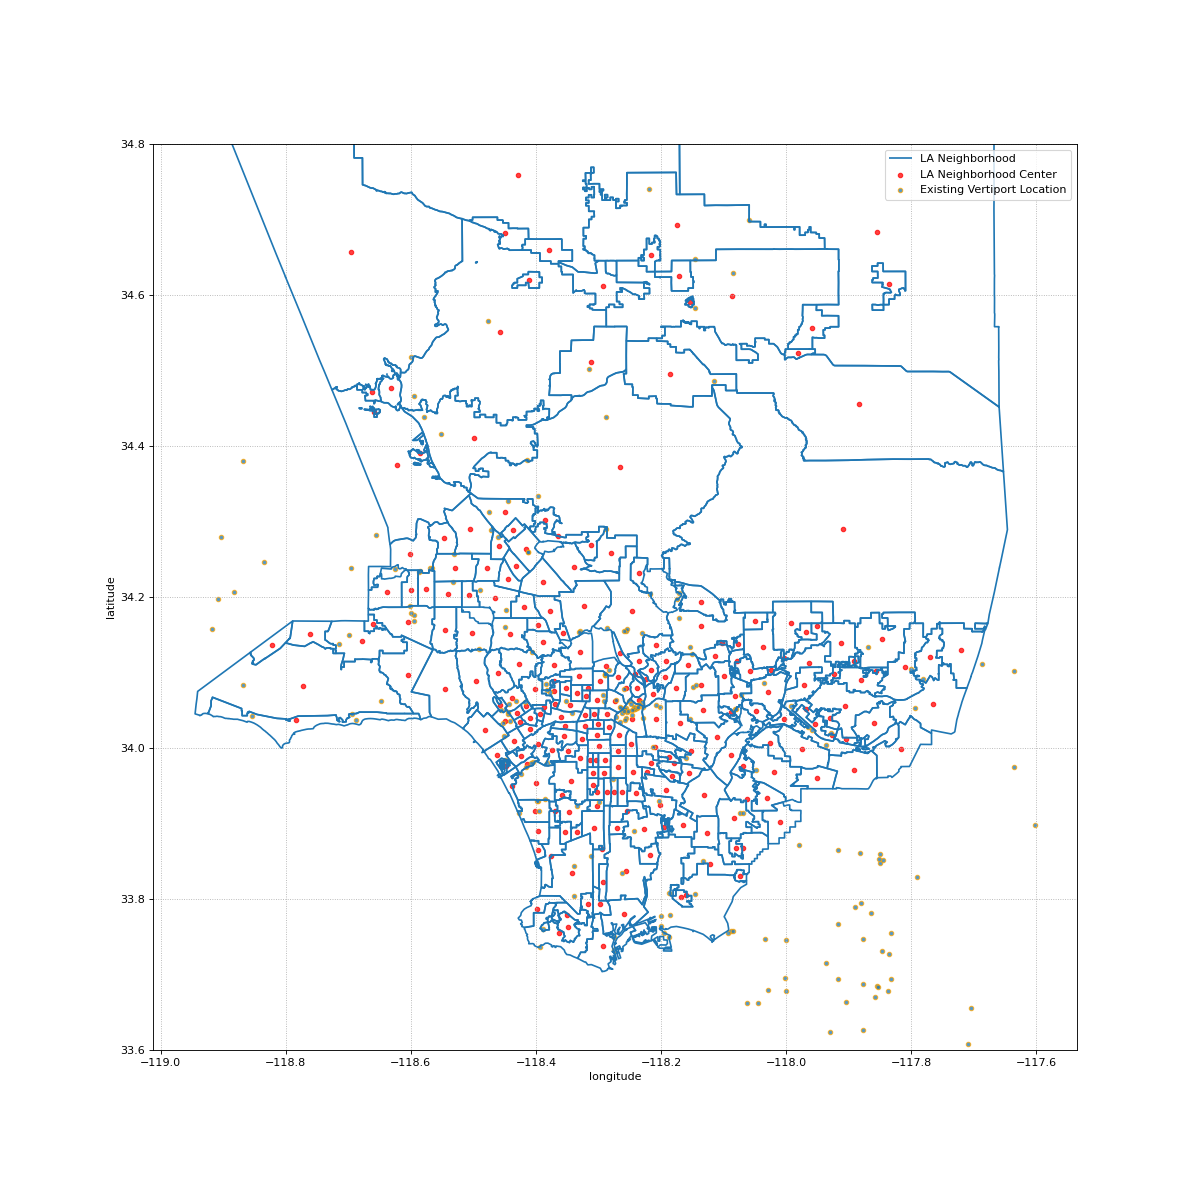
\includegraphics[width=0.8\textwidth]{proj01.png}
\vspace*{-10mm}
\caption{Los Angeles Neighborhood Centroids and Boundaries, Overlay with Available Vertiports }
\label{fig:proj01}
\end{figure}

\subsubsection{ISOMAP and Kmeans}
First construct weighted neighbor graph, given by matrix $D\in R^{m\times m}$, and
\[
D_{ij} = ||x_i - x_j||_d \qquad d \text{ is geographical distance between pair of centroids}
\]

Then, apply ISOMAP transformation on neighborhood centroids to take account for geographical distance. In order to determine optimal number of clusters for great Los Angeles area, we used Kmeans algorithm, and plot sum of squared distance vs. number of clusters, K, when K goes from 1 to 20. From Figure \ref{fig:proj02}, elbow point seems to happen between $K=5$ and $K=10$.

\begin{figure}[ht]
\centering
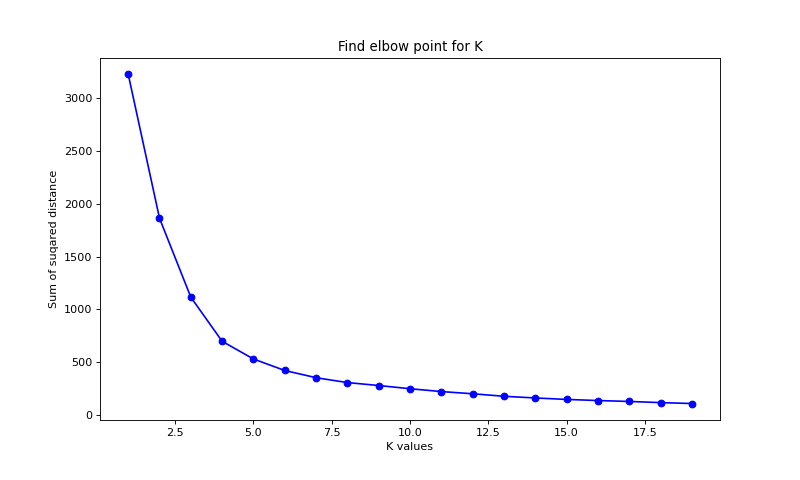
\includegraphics[width=0.8\textwidth]{proj02.png}
\vspace*{-10mm}
\caption{Find Optimal Number of Clusters}
\label{fig:proj02}
\end{figure}

Here we tried a few clustering configurations for $K=5$, $K=7$ and $K=10$, as shown in Figure \ref{fig:proj03}. Although the more clusters there are the less sum of squared distance, we believe 10 clusters is good enough to represent both urban and suburban areas. 

\begin{figure}[ht]
\centering
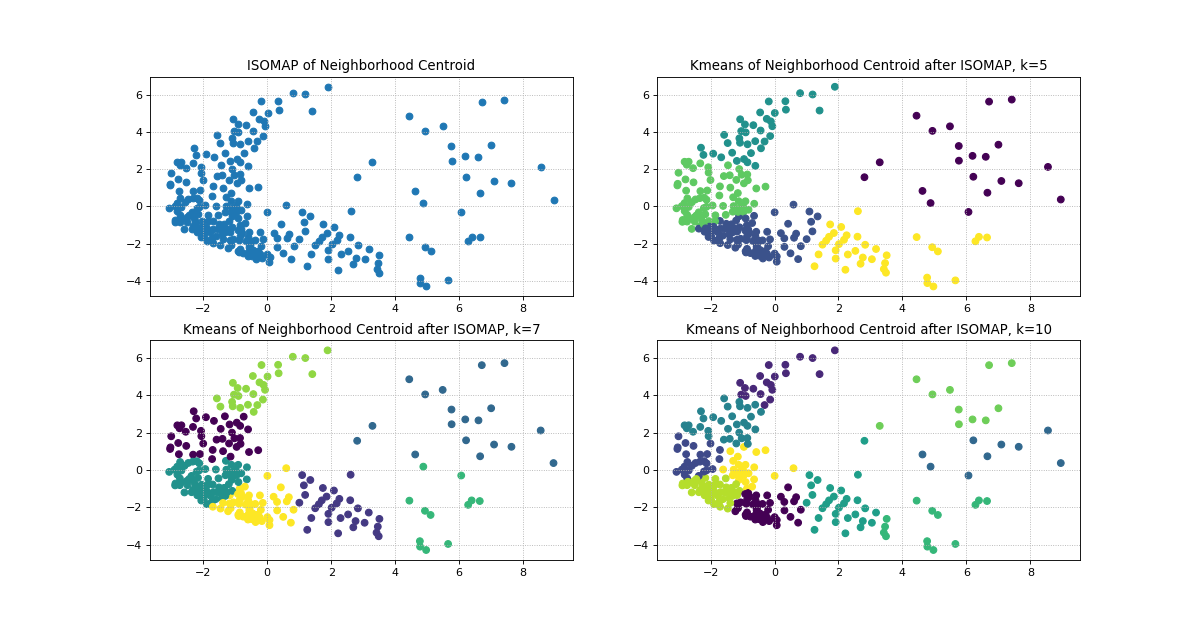
\includegraphics[width=0.9\textwidth]{proj03.png}
\vspace*{-10mm}
\caption{Different clustering results on ISOMAP of Centroids }
\label{fig:proj03}
\end{figure}

Once we established $K=10$ clusters, assign each neighborhood with its cluster label, and compute geographical cluster centers as shown in Figure \ref{fig:proj04}. Since mapping is color coded by population percentile, there are more cluster centers in most populated area, which makes sense for commuting needs.

\begin{figure}[ht]
\centering
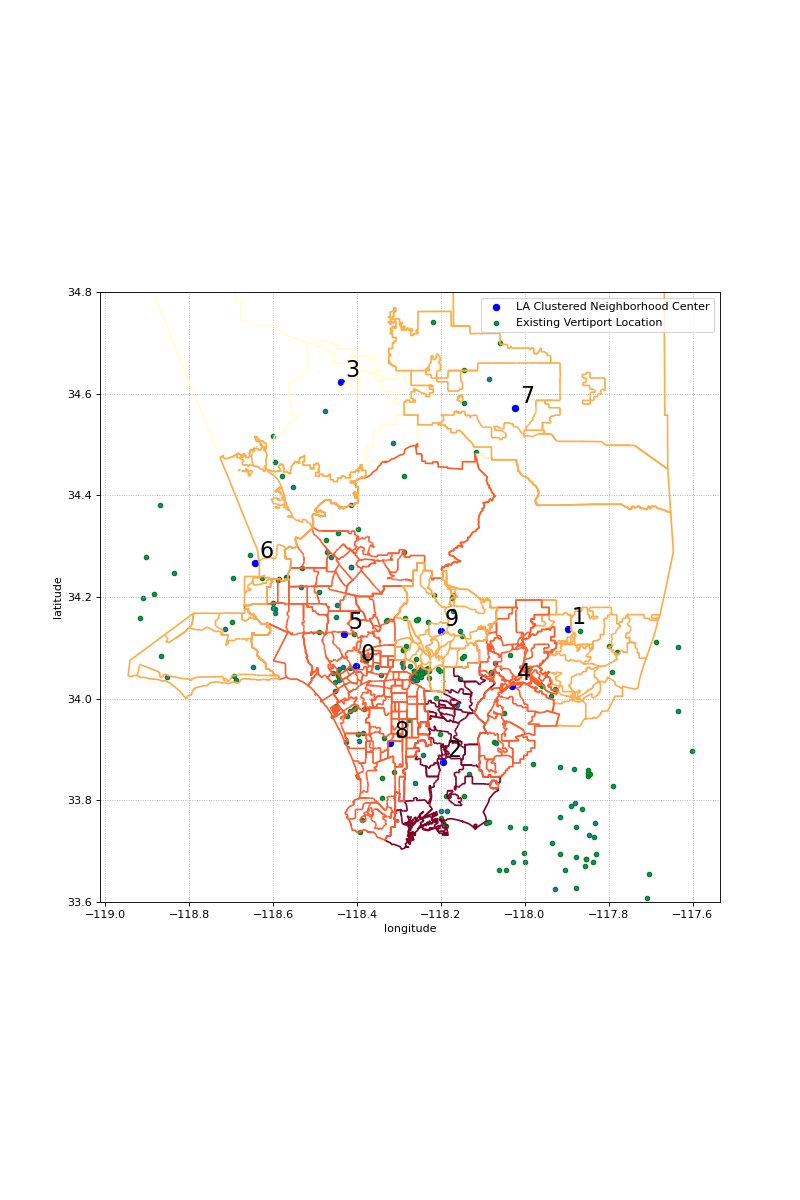
\includegraphics[width=0.8\textwidth]{proj04.png}
\vspace*{-45mm}
\caption{10 Cluster Centroids on LA Area, with Population Percentile Overlay }
\label{fig:proj04}
\end{figure}

\subsubsection{Optimization}

Assumption
\begin{enumerate}
  \item Commuters in each clusters have equal probability travel to other clusters
  \item Commuters have fixed percentage of total population
  \item Operation profit per passenger per mile is roughly estimated without large scale data
  \item All existing vertiports are available to use or rent
  \item Both existing and new vertiports have same eVTOL capacity
  \item During commute time, each eVTOL can make 3 round trips without charging
\end{enumerate}

Data
\[
\begin{split}
K& \qquad \text{Number of clusters we choose}\\
c_{ij}&  \qquad \text{Number of daily commuters between cluster $i$ and cluster $j$} \\
p_{ij}& \qquad \text{Percentage of commuter in cluster $i$ would choose eVTOL}\\
d_{ij}&  \qquad \text{geographical distance between cluster $i$ and cluster $j$} \\
P & \qquad \text{Net profit per passenger per mile} \\
V^{exist}_i & \qquad \text{Number of existing vertiport that cluster $i$ have} \\
V^{new}_i & \qquad \text{Number of new vertiport that cluster $i$ should have} \\
Cap^{eVTOL} & \qquad \text{Capacity of one eVTOL, how many commuters can one eVTOL hold} \\
Cap^{port} & \qquad \text{Capacity of one vertiport, how many eVTOL can one vertiport hold} \\
Cost^{eVTOL} & \qquad \text{how much does one eVTOL cost, depreciation life 10 years} \\
Cost^{Ve} & \qquad \text{how much does using/renting one existing vertiport cost, annually} \\
Cost^{Vn} & \qquad \text{how much does building one new vertiport cost, depreciation life 20 years} \\
N^{Ve}_i & \qquad \text{number of existing vertiport in cluster $i$} \\
N^{Vn}_i & \qquad \text{number of new vertiport in cluster $i$} \\
N^{r} & \qquad \text{number of round trips one eVTOL can make during commute hours}
\end{split}
\]

Variable
\[
x_{i}  \qquad \text{Number of eVTOL that cluster $i$ should maintain} \\
\]


Objective function is 
\[
\textbf{max} \biggl( \sum_{i=1}^K \sum_{j=1}^K c_{ij}p_{ij} d_{ij}P - \sum_{i=1}^K\Bigl( \frac{1}{10\times365}Cost^{eVTOL}x_i + \frac{1}{365}Cost^{Ve}N^{Ve}_i + \frac{1}{20\times365}Cost^{Vn}N^{Vn}_i  \Bigl)\biggl)
\]

Subject to
\[
\begin{split}
x_i  \geq 0 &\qquad \text{number of eVTOL that each vertiport have cannot be zero}\\
Cap^{eVTOL}N^{r}x_i \geq \sum_{j=1}^K c_{ij}p_{ij} &\qquad \text{total eVTOL capacity of cluster $i$ can satisfy all eVTOL commute needs} \\
Cap^{port}(N^{Ve}_i+N^{Vn}_i) \geq x_i &\qquad  \text{total vertiport capacity of cluster $i$ can hold all eVTOL in cluster $i$} \\
\end{split}
\]

\begin{table}[h!]
\centering
\caption{Table for constant parameters}
\begin{tabular}{|c c l|} 
 \hline
 Constant & Value & Description \\ [0.5ex] 
 \hline\hline
 $K$ & 10 & Number of clusters we choose \\
 $p_{ij}$ & $5\%\times 2.5\%$ & total commute is 5\% of population, eVTOL commute is 2.5\% of total commute \\
 $N^r$ & 3 & Number of round trip one eVTOL can make during commute hours\\
 $P$ & \$0.5 & Net profit per passenger per mile \\ 
 $Cap^{eVTOL}$ & 4 & Capacity of one eVTOL\\
 $Cap^{port}$ & 8 & Capacity of one vertiport\\
 $Cost^{eVTOL}$ & \$100,000 & One eVTOL cost, depreciation life is 10 years\\
 $Cost^{Ve}$ & \$12,000 & Annual renting cost of one existing vertiport (Cap 8 eVTOL) \\
 $Cost^{Vn}$ & \$200,000 & Building cost of one new vertiport (Cap 8 eVTOL), depreciation life is 20 years \\ [1ex] 
 \hline
\end{tabular}
\label{table:proj01}
\end{table}

Future refinement:
\begin{enumerate}
  \item Commuters in each clusters have dynamic probability travel to other clusters
  \item Commuters' percentage of total population is related to other factors, like wealth, race, age, etc.
  \item Further explore availability of existing vertiports
\end{enumerate}

User python package Pulp to solve optimization problem.

\section{Final Results}

\begin{table}[h!]
\centering
\caption{Optimization Results}
\begin{tabular}{|c c c c c c|} 
 \hline
cluster\_label& existing\_vertiport&	total\_commute&	total\_prof&	new\_vertiport&	eVTOL\_number \\ [0.5ex] 
 \hline\hline
0&	22	& 2,398& 23,418	& 3	& 200 \\
1&	4&	1,948&	26,239&	17&	163\\
2&	18&	2,994&	36,338&	14&	250\\
3&	3&	1,210&	26,221&	10&	101\\
4&	14&	2,301&	25,531&	10&	192\\
5&	12&	2,317&	23,761&	13&	194\\
6&	19&	1,516&	23,336&	0&	127\\
7&	5&	1,469&	29,907&	11&	123\\
8&	13&	2,925&	33,054&	18&	244\\
9&	49&	2,224&	20,626&	0&	186\\ [1ex] 
 \hline
\end{tabular}
\label{table:proj02}
\end{table}

Total daily profit is \$211,806.34


\section{Evaluation}




\pagebreak

\begin{appendix}
  \listoffigures
  \listoftables
\end{appendix}

\end{document}

